\section{Result}
Consider a QHO described by the Hamiltonian in Eq. \eqref{eq:hamiltonian} which is coupled to a thermal bath with temperature $T$. If the oscillator's position quadrature is also continuously measured the evolution of the system can be described by the master equation in Eq. \eqref{eq:masterMeas} using the Lindblad operators mentioned in Sec. \ref{sec:mastereq}. We want to solve for the equations of motions when measuring for the position quadrature
\begin{align}
    \dt\expval{\xop^2} &= \tr(\xop^2 \dt \dmatrix)\label{eq:x2}, \\
    \dt\expval{\pop^2} &= \tr(\pop^2 \dt \dmatrix)\label{eq:p2},\\
    \dt\expval{\acomm{\xop}{\pop}} &= \tr(\acomm{\xop}{\pop} \dt \dmatrix). \label{eq:xp}
\end{align}
Solving these equations yields the following EOM
\begin{align}
    \dt\expval{\xop^2} &= - \gamma \expval{\xop^2} + \frac{1}{m}\expval{\acomm{\xop}{\pop}} + \frac{\gamma \hbar}{m\omega}(\nbar + 1/2),\\
    \dt\expval{\pop^2} &= -\gamma \expval{\pop^2} - m\omega^2 \expval{\acomm{\xop}{\pop}} + \gamma m \omega\hbar (\nbar + 1/2) + \lambda \hbar^2,\\
    \dt\expval{\acomm{\xop}{\pop}} &= -\gamma \expval{\acomm{\xop}{\pop}} + 2 m \omega^2 \expval{\xop^2} - \frac{2}{m} \expval{\pop^2}
\end{align}
for more detailed calculations see App. \ref{app:eom}. Performing a change of variable to make the equations dimensionless
\begin{equation}
    \tilde{x} = \sqrt{\frac{m\omega}{\hbar}} x \quad \text{and} \quad \tilde{p} = \sqrt{\frac{1}{m \omega \hbar}} p ,
\end{equation}
we can solve for the steady state. By introducing the quality factor $Q = \omega / \gamma$ we obtain the steady state solutions
\begin{align}
    \expval{\tilde{x}^2} &= (\nbar + 1/2) + \frac{\lambda \hbar}{m \omega^2} \frac{2 Q^3}{4Q^2 - 1},\\
    \expval{\tilde{p}^2} &= (\nbar + 1/2) + \frac{\lambda \hbar}{m \omega^2} \left( Q - \frac{2Q^3}{4Q^2 - 1} \right),\\
    E &= \expval{\tilde{H}} = \frac{\hbar \omega}{2} \left( \expval{\tilde{p}^2} + \expval{\tilde{x}^2} \right).
\end{align}
Plotting the energy of the system 

\begin{figure}[ht]
    \centering
    \begin{subfigure}[t]{0.48\textwidth}
        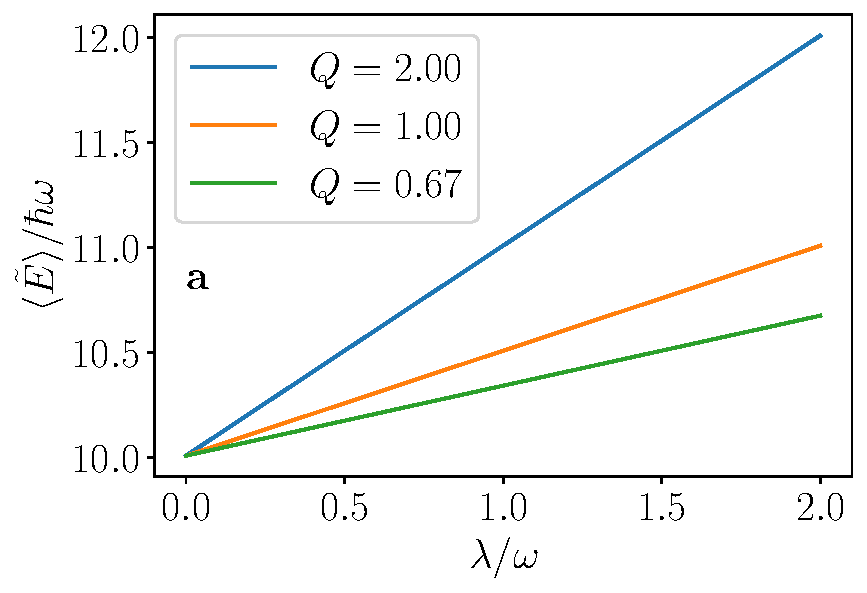
\includegraphics[width=\textwidth]{figures/E_vs_lambda}
        \caption{The energy plotted against $\lambda / \omega$ with varying $Q$.}
        \label{fig:E_vs_lambda}
    \end{subfigure}
    \hfill
    \begin{subfigure}[t]{0.48\textwidth}
        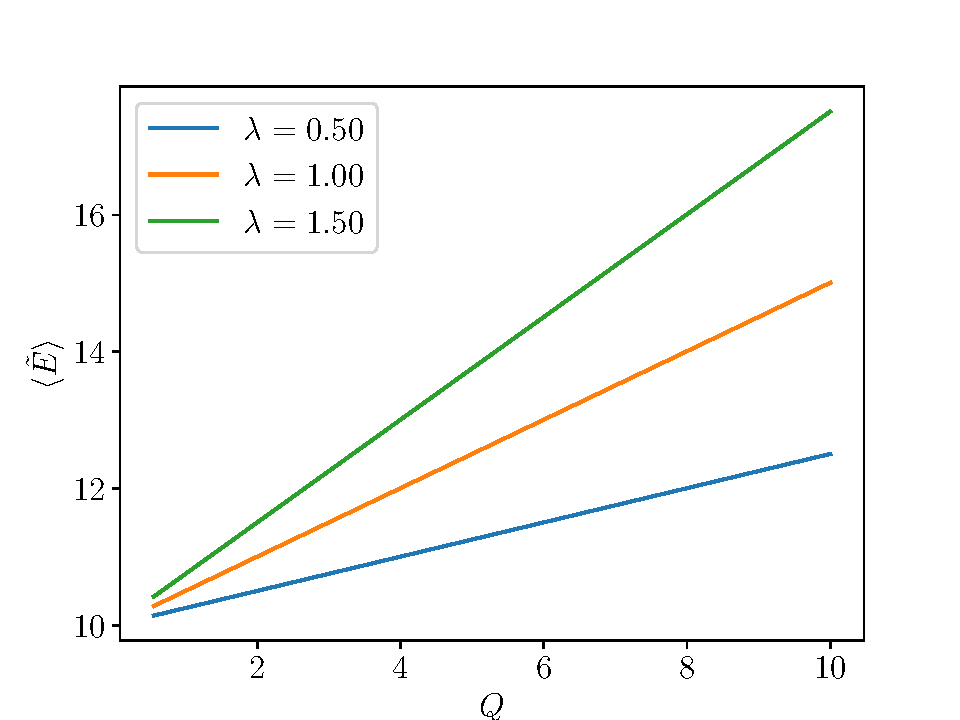
\includegraphics[width=\textwidth]{figures/E_vs_Q}
        \caption{The energy plotted against $Q$ with varying $\lambda$.}
        \label{fig:E_vs_Q}
    \end{subfigure}
    \caption{The energy plotted against $\lambda / \omega$ and $Q$ with the parameters $k_\mathrm{B}T = 10$ and $\omega = 1$. This gives $\nbar + 1/2 \approx 10 $}.
    \label{fig:E_plots}
\end{figure}
Looking at Fig. \ref{fig:E_plots} one can see that a stronger measurement correlates to the system steady state increasing in energy. It is also noteworthy that the same applies for the quality factor. Thus, by continuously measuring the system we add energy into it, which make the steady state higher in energy than what the thermal effects from the bath would otherwise place it. 